% CVPR 2026 Paper Template
\documentclass[10pt,twocolumn,letterpaper]{article}

% \usepackage{cvpr}              % camera-ready
\usepackage{cvpr}        % review version (with ruler)
% \usepackage[pagenumbers]{cvpr} % arXiv version

\usepackage{graphicx}
\usepackage{amsmath}
\usepackage{amssymb}
\usepackage{booktabs}
\usepackage{multirow}
\usepackage{subcaption}
\usepackage{microtype}
\usepackage{tikz}
\usetikzlibrary{arrows.meta, positioning, fit, backgrounds, shapes.geometric, calc}

\definecolor{cvprblue}{rgb}{0.21,0.49,0.74}
\usepackage[pagebackref,breaklinks,colorlinks,allcolors=cvprblue]{hyperref}

\def\paperID{*****}
\def\confName{CVPR}
\def\confYear{2026}

\title{AudioConditioner: Knowledge Distillation for\\
Efficient Scene-Conditioned Background Music Generation}

\author{Keyvan Attarian\\
\'Ecole Polytechnique\\
{\tt\small keyvan.attarian@polytechnique.edu}
\and
Baptiste Arnaudo\\
\'Ecole Polytechnique\\
{\tt\small baptiste.arnaudo@polytechnique.edu}
}

\begin{document}
\maketitle

% -----------------------------------------------------------------------
\begin{abstract}
We present \textbf{AudioConditioner}, a multimodal pipeline that generates
semantically aligned background music from a text scene description or an
image. Our key contribution is a lightweight \emph{descriptor bridge} -- a multi-task MLP trained via synthetic distillation from a 7B-parameter LLM -- that maps frozen CLAP~\cite{elizalde2023clap} embeddings to a structured 12-attribute \emph{MusicDescriptor} intermediate representation. At inference, the LLM is replaced entirely, enabling fast scene-to-music
generation at a fraction of the cost. The MusicDescriptor encodes musically-grounded attributes (mood, energy, valence, tempo, instrumentation, production style, and more) that are serialised into a natural-language prompt conditioning a frozen text-to-audio diffusion model (Stable Audio Open~\cite{evans2024stable}). A CLAP-based re-ranking step then selects the best among $N$ candidates. On a 100-scene benchmark, the distilled model achieves a mean CLAP cosine similarity of \textbf{0.38}, outperforming direct LLM inference at runtime (0.35) while reducing inference-time parameters by three orders of magnitude. We further demonstrate three downstream applications: ambient music from images, adaptive audiobook narration with a synchronised background score, and image-to-video with a matching soundtrack.
\end{abstract}

% -----------------------------------------------------------------------
\section{Introduction}
\label{sec:intro}

Background music fundamentally shapes the emotional experience of film, games,
podcasts, and audiobooks.
Yet composing scene-appropriate music requires significant expertise, and
manually selecting tracks for every new scene is prohibitively slow.
\emph{Generating} music that is semantically consistent with a given visual or
textual scene is therefore both practically valuable and scientifically
challenging.

Recent text-to-audio diffusion models~\cite{evans2024stable, liu2023audioldm2,
copet2023simple} can synthesise high-quality music from natural-language
prompts.
The remaining bottleneck is \emph{semantic bridging}: translating an
unstructured scene description or image into the rich, musically-specific
language these models require.
Existing approaches either prompt a large LLM at every inference
step~\cite{liu2023audioldm2, agostinelli2023musiclm} -- slow and
resource-intensive -- or train end-to-end models that collapse the intermediate
representation, sacrificing interpretability and user control.

We propose a different strategy: \textbf{two-phase knowledge distillation
through a structured intermediate representation}. In Phase~1, a 7B-parameter teacher LLM (Qwen2.5~\cite{qwen2025qwen25}) labels a large procedurally-generated scene corpus with structured \emph{MusicDescriptor} JSON objects \emph{offline}. In Phase~2, a tiny student MLP is trained to predict these descriptors from frozen CLAP embeddings. At inference, no LLM is needed: the student runs in milliseconds.

The \emph{MusicDescriptor} is the linchpin of the approach.
It encodes 12 musically-grounded attributes that a \texttt{prompt()} method
serialises into six natural-language sentences, conditioning Stable Audio
Open~\cite{evans2024stable}.
This decomposition is \emph{interpretable} -- each attribute can be inspected or manually overridden -- and \emph{composable} across applications.

\noindent\textbf{Contributions:}
\begin{enumerate}
  \item A structured \emph{MusicDescriptor} schema bridging scene understanding
        and audio synthesis.
  \item A two-phase knowledge-distillation framework replacing 7B-parameter LLM
        inference with a $<$1M-parameter MLP.
  \item A CLAP-based self-supervised re-ranking mechanism.
  \item Three demonstrated downstream applications.
  \item Quantitative benchmarks showing the distilled model outperforms direct
        LLM inference on CLAP similarity.
\end{enumerate}

% -----------------------------------------------------------------------
\section{Related Work}
\label{sec:related}

\paragraph{Text-to-music generation.}
MusicLM~\cite{agostinelli2023musiclm} and MusicGen~\cite{copet2023simple}
generate music from text prompts using language models over discrete audio
tokens.
AudioLDM~2~\cite{liu2023audioldm2} and Stable Audio Open~\cite{evans2024stable}
adopt latent diffusion, achieving higher audio fidelity and longer generation
windows.
All these models accept free-form text; we focus on \emph{automatically
constructing} that text from scenes.

\paragraph{Multimodal scene-to-audio.}
Generating sound from video~\cite{su2023physics, mo2023foleycrafter} or
images~\cite{iashin2021taming} has been studied for sound effects; background
music with scene-level semantics is less explored.
V-MusProd~\cite{zhuo2023video} and CMT~\cite{di2021video} condition music
generation on video features but require audio-visual paired training data and
generate short clips.
Our approach requires no such paired data: the pairing is created synthetically
via the teacher LLM.

\paragraph{Knowledge distillation.}
Hinton \etal~\cite{hinton2015distilling} introduced knowledge distillation for
model compression; subsequent works distil LLMs into smaller models for
classification~\cite{sanh2019distilbert} and
generation~\cite{kim2016sequence}.
Our setting is distinctive: the teacher produces \emph{structured outputs}
(JSON schema), and the student is a multi-task MLP trained on frozen
pretrained embeddings, making training very data-efficient.

\paragraph{Contrastive language-audio pretraining (CLAP).}
CLAP~\cite{elizalde2023clap} learns a shared embedding space for text and
audio via contrastive pretraining, analogous to CLIP~\cite{radford2021clip}
for vision-language.
We use CLAP both as the scene encoder (input to the student MLP) and as a
zero-shot evaluator for re-ranking and benchmarking.

% -----------------------------------------------------------------------
\section{Method}
\label{sec:method}

\subsection{System overview}

\Cref{fig:pipeline} gives an overview of the full inference pipeline.
Given a text scene description (or an image first captioned by
BLIP~\cite{li2022blip}), a frozen CLAP text encoder produces a 512-dimensional
semantic embedding.
This embedding is passed to the \emph{descriptor bridge} -- the only trained
component -- which outputs a \emph{MusicDescriptor} object.
The MusicDescriptor's \texttt{prompt()} method builds a natural-language music
prompt, which conditions Stable Audio Open to generate $N$ candidate waveforms.
Finally, a CLAP audio encoder re-ranks the candidates by cosine similarity
with the original scene embedding, and the best waveform is returned.

\begin{figure*}[t]
\centering
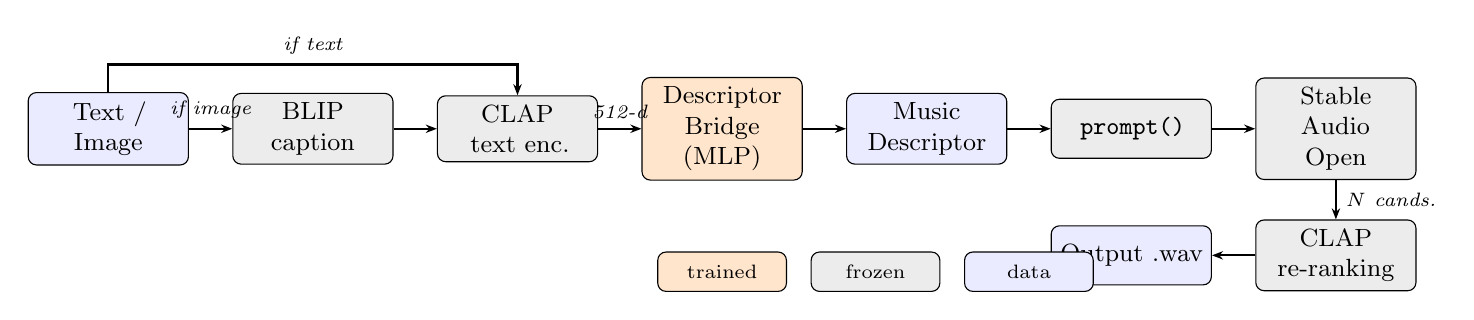
\begin{tikzpicture}[
  node distance=0.45cm and 0.55cm,
  block/.style={rectangle, draw, rounded corners=3pt, fill=blue!8,
                text centered, minimum height=0.75cm, font=\small,
                text width=1.8cm},
  frozen/.style={rectangle, draw, rounded corners=3pt, fill=gray!15,
                 text centered, minimum height=0.75cm, font=\small,
                 text width=1.8cm},
  trained/.style={rectangle, draw, rounded corners=3pt, fill=orange!20,
                  text centered, minimum height=0.75cm, font=\small,
                  text width=1.8cm},
  arr/.style={-{Stealth[length=4pt]}, thick},
  label/.style={font=\scriptsize\itshape}
]
% Input
\node[block] (input) {Text / Image};
\node[frozen, right=of input] (blip) {BLIP\\caption};
\node[frozen, right=of blip] (clap_enc) {CLAP\\text enc.};
\node[trained, right=of clap_enc] (mlp) {Descriptor\\Bridge (MLP)};
\node[block, right=of mlp] (desc) {Music\\Descriptor};
\node[frozen, right=of desc] (prompt) {\texttt{prompt()}};
\node[frozen, right=of prompt] (sao) {Stable Audio\\Open};
\node[frozen, below=0.5cm of sao] (rerank) {CLAP\\re-ranking};
\node[block, left=of rerank] (out) {Output .wav};

\draw[arr] (input) -- node[above,label]{if image} (blip);
\draw[arr] (blip) -- (clap_enc);
\draw[arr] (input.north) -- ++(0,0.35) -| node[above,label,pos=0.25]{if text} (clap_enc.north);
\draw[arr] (clap_enc) -- node[above,label]{512-d} (mlp);
\draw[arr] (mlp) -- (desc);
\draw[arr] (desc) -- (prompt);
\draw[arr] (prompt) -- (sao);
\draw[arr] (sao) -- node[right,label]{$N$ cands.} (rerank);
\draw[arr] (rerank) -- (out);

% Legend
\node[trained, below=0.9cm of mlp, text width=1.4cm, minimum height=0.5cm] (leg_t) {\scriptsize trained};
\node[frozen,  right=0.3cm of leg_t, text width=1.4cm, minimum height=0.5cm] (leg_f) {\scriptsize frozen};
\node[block,   right=0.3cm of leg_f, text width=1.4cm, minimum height=0.5cm] (leg_n) {\scriptsize data};

\end{tikzpicture}
\caption{AudioConditioner inference pipeline. Grey = frozen pretrained model;
orange = the only trained component (the descriptor bridge MLP).}
\label{fig:pipeline}
\end{figure*}

\subsection{MusicDescriptor}

The \emph{MusicDescriptor} is the structured intermediate representation at the
core of our system.
It encodes 12 musically-grounded attributes (\cref{tab:descriptor}):
five single-label classification attributes (key mode, rhythm style, structure,
dynamics profile), seven multi-label attributes (mood, instrumentation,
production style), and five regression attributes (energy, valence, tempo,
harmonic tension, texture density).
Together these cover perceptual, harmonic, rhythmic, timbral, and structural
dimensions of a music piece.

The \texttt{prompt()} method serialises all 12 attributes into six sentences,
\eg: \textit{``The piece has an ominous, tense mood. Energy: 0.82 (very
energetic). Tempo: 142 BPM, driving rhythm, gradual crescendo. Key mode:
minor. Instrumentation: low strings, war drums, cinematic percussion.
Production style: cinematic, reverb heavy.''}

\begin{table}[t]
\caption{MusicDescriptor attributes. \textit{CLS}: single-label
  classification; \textit{ML}: multi-label; \textit{REG}: regression.}
\label{tab:descriptor}
\centering\small
\begin{tabular}{@{}llr@{}}
\toprule
Attribute & Type & \# classes / range \\
\midrule
Mood              & ML  & 20 labels \\
Energy            & REG & $[0, 1]$ \\
Valence           & REG & $[0, 1]$ \\
Tempo             & REG & $[50, 180]$ BPM \\
Key mode          & CLS & 3 (maj / min / amb.) \\
Harmonic tension  & REG & $[0, 1]$ \\
Texture density   & REG & $[0, 1]$ \\
Instrumentation   & ML  & 23 labels \\
Rhythm style      & CLS & 7 \\
Structure         & CLS & 5 \\
Production style  & ML  & 10 labels \\
Dynamics profile  & CLS & 5 \\
\bottomrule
\end{tabular}
\end{table}

\subsection{Descriptor bridge architecture}

The descriptor bridge (\emph{TwoDeepDescriptor}) maps a 512-d CLAP
embedding to a MusicDescriptor via a shared backbone and 13 task-specific
output heads:

\begin{equation}
  \mathbf{h} = \mathrm{ReLU}(W_3\,\mathrm{ReLU}(W_2\,\mathrm{ReLU}(W_1\,\mathbf{z})))
  \label{eq:backbone}
\end{equation}
where $\mathbf{z}\in\mathbb{R}^{512}$ is the CLAP embedding and each $W_i$
projects to dimension 256.
Each output head appends a second linear-ReLU-linear block projecting
$\mathbf{h}$ to the appropriate output dimension.

Classification heads output a softmax distribution; multi-label heads use
top-$p$ thresholding (default $p{=}0.1$) with an argmax fallback.
Regression heads apply a sigmoid and, for tempo, rescale to $[50, 180]$ BPM.

The total parameter count is approximately \textbf{640\,000}---three orders of
magnitude smaller than the 7B-parameter Qwen2.5 teacher.

\subsection{Training}

\paragraph{Phase~1 -- Procedural scene corpus.}
The scene generator constructs up to 160\,000
short scenes by combining 20 characters $\times$ 20 characteristics $\times$
20 settings $\times$ 21 events (\eg, \textit{``A driven monk inside a
candlelit cathedral watches a kingdom fall''}).
Qwen2.5-7B-Instruct is prompted with a strict JSON schema and assigns a
MusicDescriptor to each scene at temperature 0.2.
The resulting dataset is stored as JSONL with $\sim$120\,000 valid entries.

\paragraph{Phase~2 -- Novel chunk fine-tuning.}
For the ReadMusic application, public-domain short stories such as Grimm's are chunked into ${\le}80$-word
paragraphs. The teacher LLM is prompted again -- now with narrative context from preceding chunks -- to produce \emph{temporally coherent} MusicDescriptor sequences. Fine-tuning on these chunks produces a checkpoint that internalises emotional arc and narrative momentum.

\paragraph{Loss.}
The training loss sums per-attribute terms:
\begin{equation}
  \mathcal{L} = \sum_{k \in \mathcal{C}} \mathrm{CE}(\hat{y}_k, y_k)
              + \sum_{k \in \mathcal{R}} \mathrm{MSE}(\hat{y}_k, y_k)
  \label{eq:loss}
\end{equation}
where $\mathcal{C}$ is the set of classification attributes and $\mathcal{R}$
the regression attributes.
The model is trained with Adam ($\eta{=}5{\times}10^{-4}$), batch size 64,
for 50 epochs on an 80/20 train/val split.
\Cref{fig:train_loss} and \Cref{fig:validation_loss} show convergence curves.

\begin{figure}[t]
  \centering
  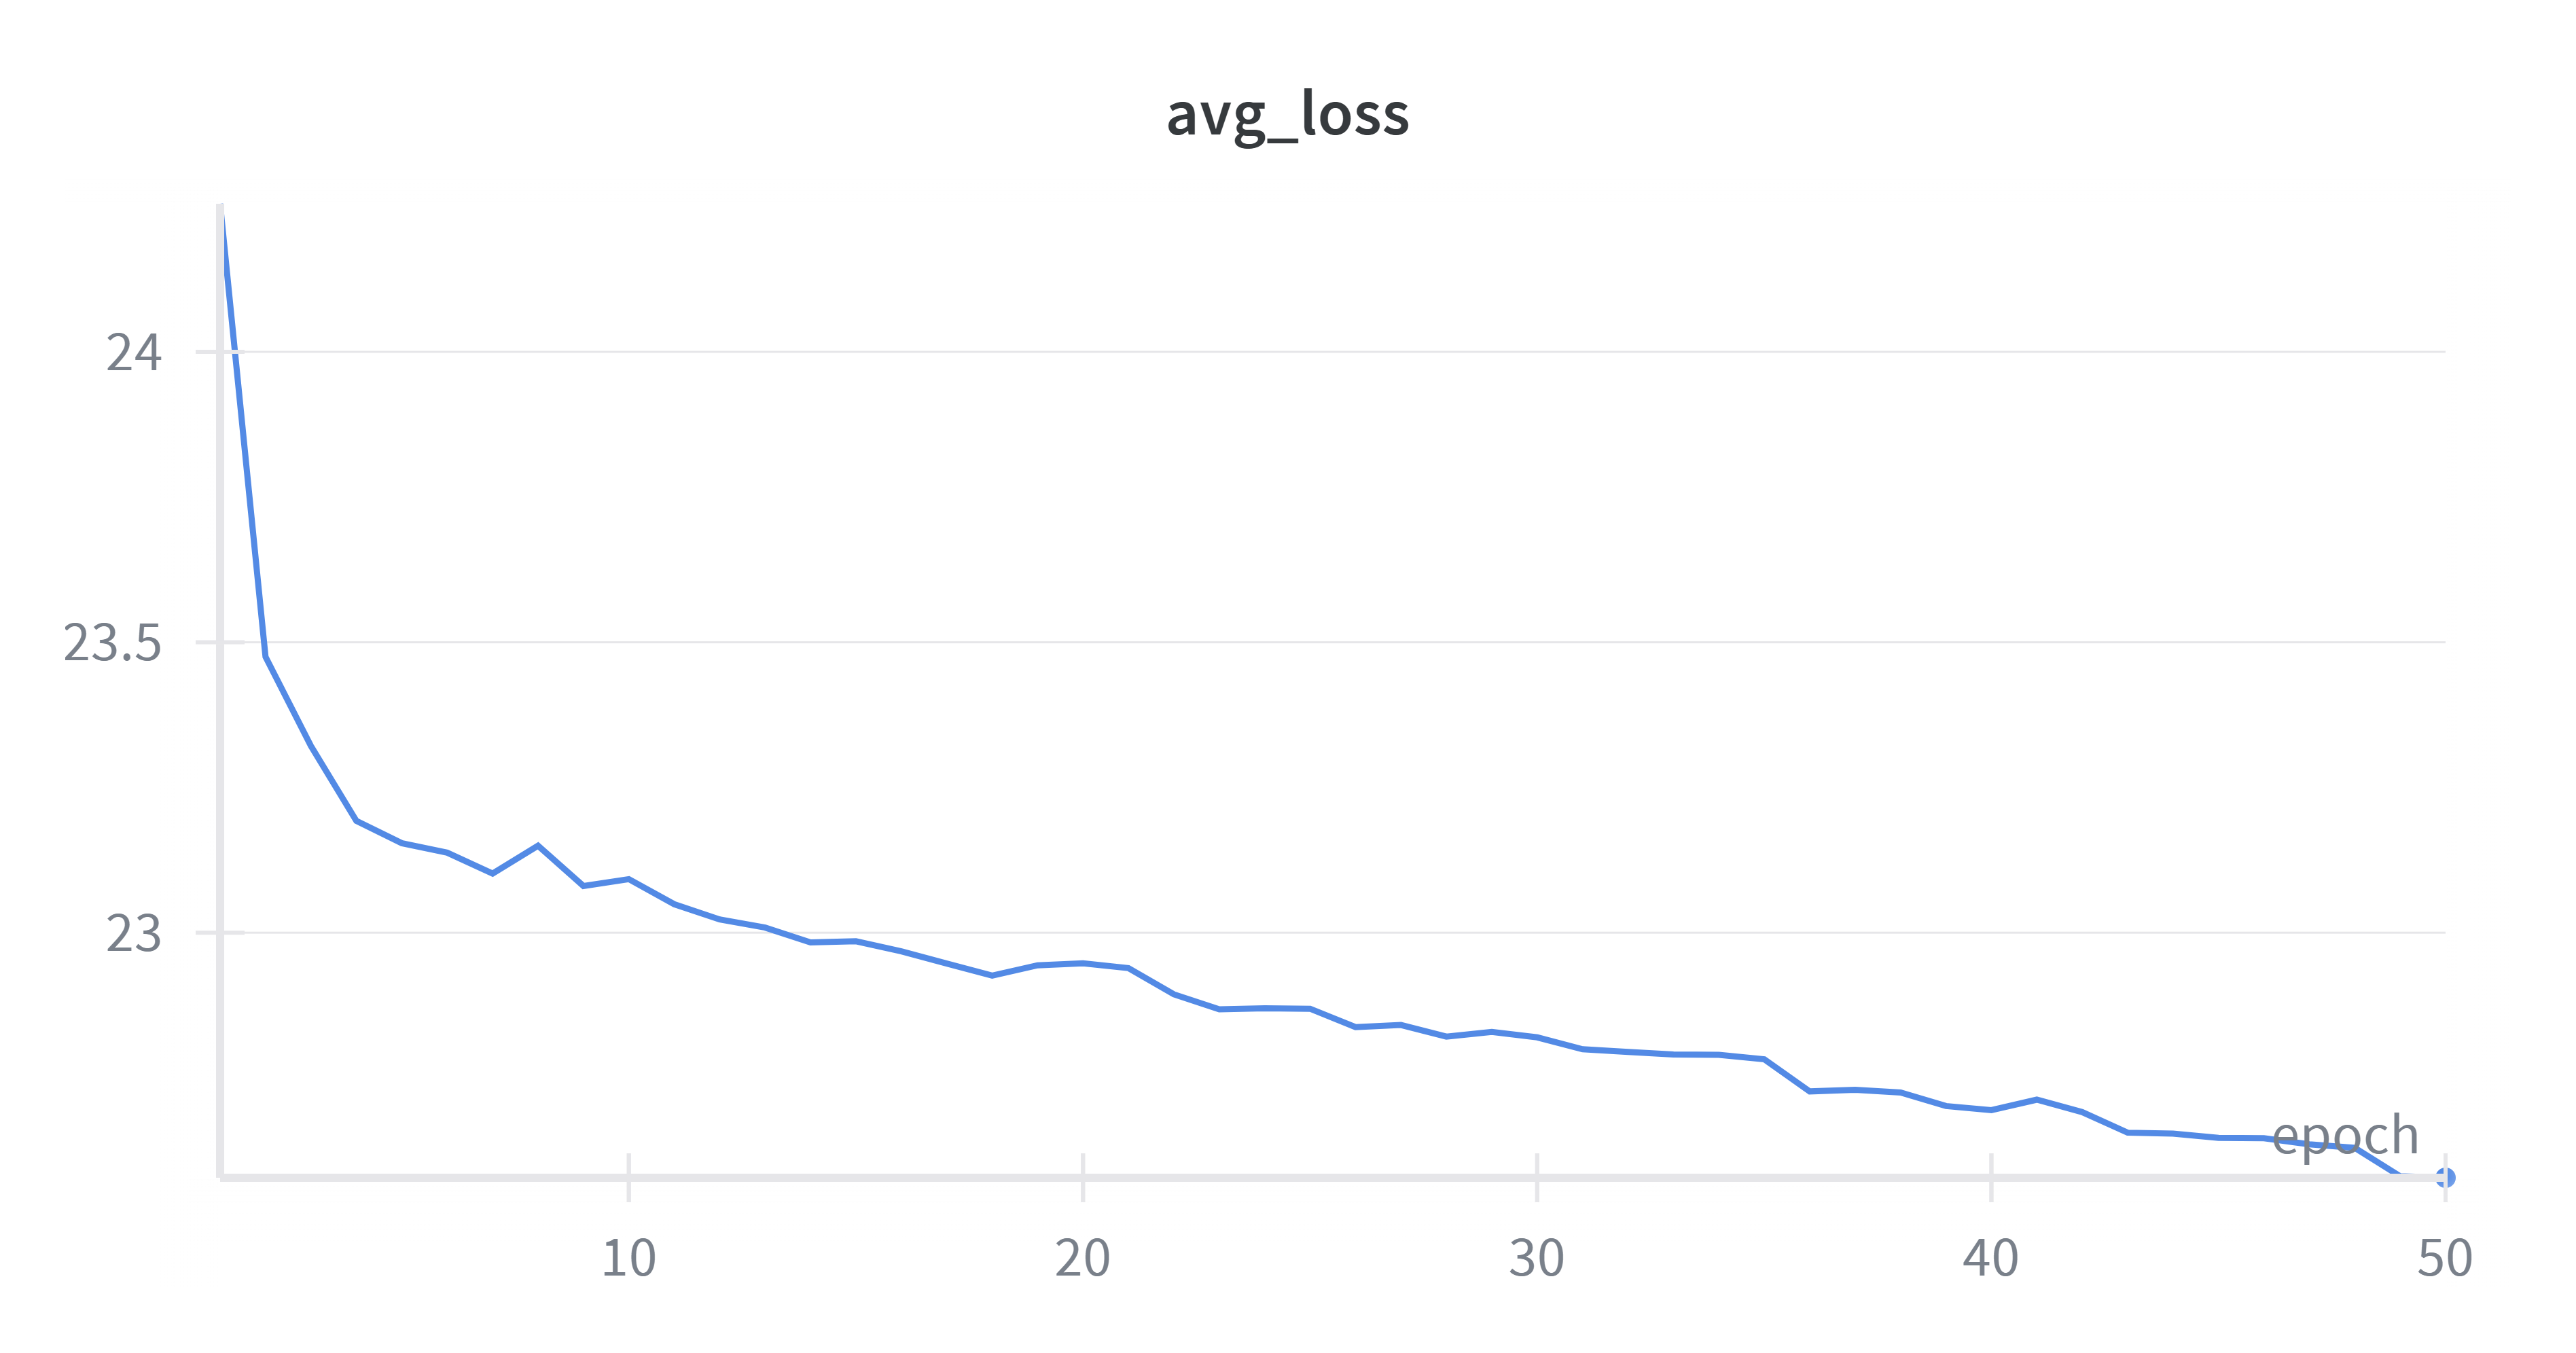
\includegraphics[width=\linewidth]{figures/avg_loss.png}
  \caption{Training loss curve over 50 epochs.}
  \label{fig:train_loss}
\end{figure}

\begin{figure}[t]
  \centering
  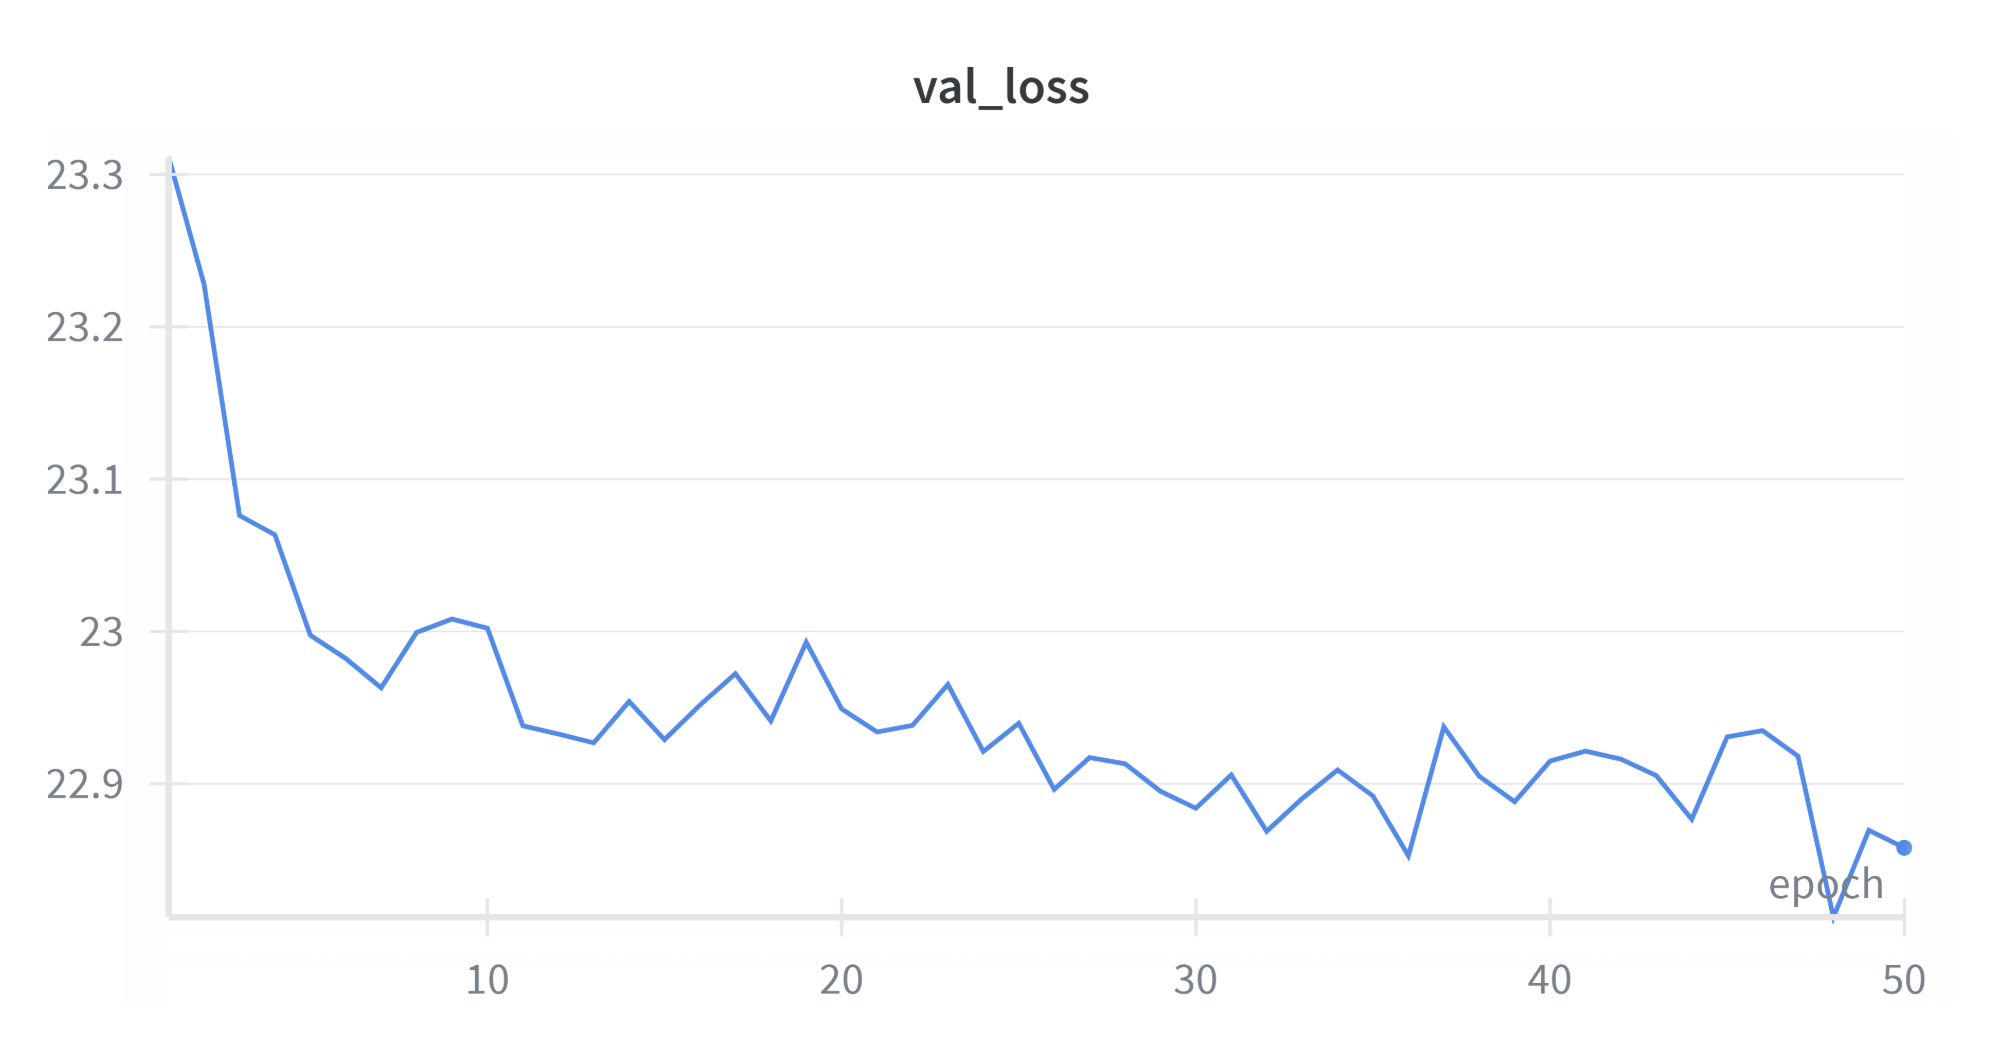
\includegraphics[width=\linewidth]{figures/val_loss.png}
  \caption{Validation loss curve over 50 epochs.}
  \label{fig:validation_loss}
\end{figure}

\subsection{CLAP re-ranking}

Given $N$ generated waveforms $\{a_i\}$, the system selects
\begin{equation}
  i^* = \arg\max_i \;\cos\!\left(\phi_\text{txt}(s),\;\phi_\text{aud}(a_i)\right)
  \label{eq:rerank}
\end{equation}
where $s$ is the input scene text, $\phi_\text{txt}$ the CLAP text encoder,
and $\phi_\text{aud}$ the CLAP audio encoder.
This is a quality improvement that leverages the same frozen model
used during training, incurring no additional learned parameters. Its only cost is an increased inference time.

% -----------------------------------------------------------------------
\section{Experiments}
\label{sec:experiments}

\subsection{Benchmark setup}

We evaluate semantic alignment using \textbf{CLAP cosine similarity} between
the input scene text and the generated audio, computed over 100 held-out scenes
from a public-domain novel chunk test set.
Three systems are compared:

\begin{itemize}
  \item \textbf{AudioConditioner}: CLAP $\to$ student MLP $\to$ MusicDescriptor
        $\to$ Stable Audio Open.
  \item \textbf{LLM baseline}: Qwen2.5-7B inference at test time $\to$
        MusicDescriptor $\to$ Stable Audio Open.
  \item \textbf{Random baseline}: random sampling from all vocabulary lists
        $\to$ MusicDescriptor $\to$ Stable Audio Open.
\end{itemize}

All three use the same Stable Audio Open backbone ($N{=}1$ candidate, 50 DDIM
steps, 47-second clips) and CLAP evaluator to ensure a fair comparison.

\subsection{Results}

\Cref{tab:results} and \cref{fig:scores} summarise the benchmark results.
AudioConditioner achieves a mean CLAP cosine similarity of \textbf{0.38},
outperforming the LLM baseline (0.35) by $+0.03$ absolute and far exceeding
the random baseline (0.27).

\begin{table}[t]
\caption{CLAP cosine similarity on the 100-scene benchmark (higher is better).
The distilled model outperforms the 7B-parameter LLM baseline at inference time.}
\label{tab:results}
\centering\small
\begin{tabular}{@{}lcc@{}}
\toprule
Method & Mean sim. & $\Delta$ vs.\ LLM \\
\midrule
Random baseline              & 0.27 & $-$0.08 \\
LLM baseline (Qwen2.5-7B)   & 0.35 & \phantom{$+$}--- \\
\textbf{AudioConditioner}    & \textbf{0.38} & $+$0.03 \\
\bottomrule
\end{tabular}
\end{table}

\begin{figure}[t]
  \centering
  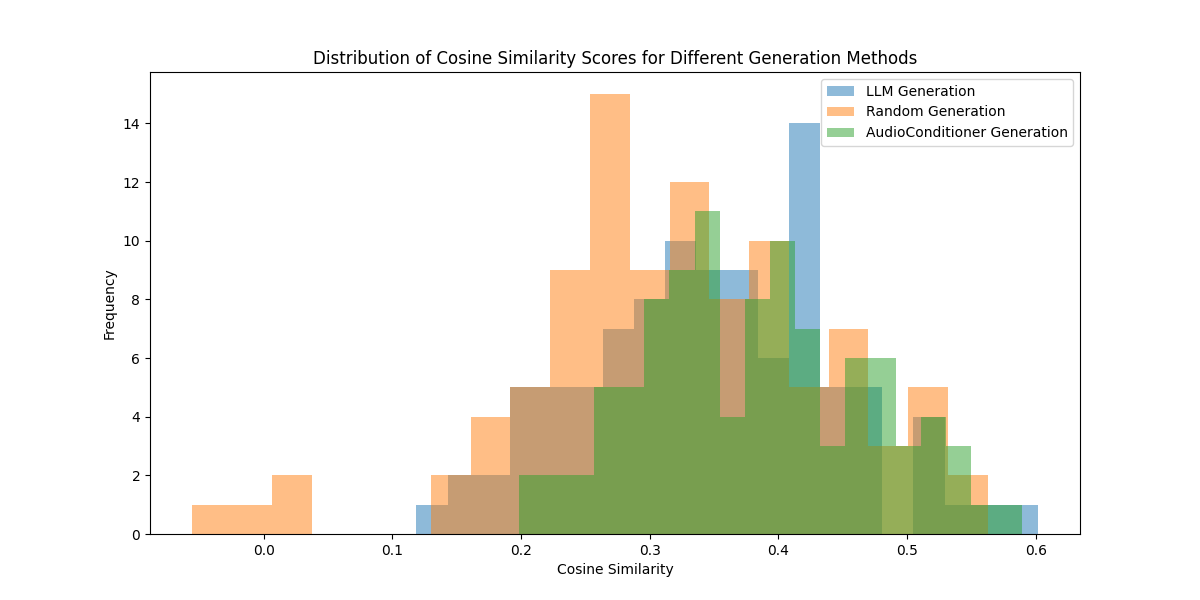
\includegraphics[width=1.1\linewidth]{figures/score_distributions.png}
  \caption{Distribution of per-scene CLAP cosine similarities.
  AudioConditioner (orange) is consistently higher than the LLM baseline
  (blue) and the random baseline (green).}
  \label{fig:scores}
\end{figure}

\subsection{Discussion}

The student MLP outperforming the 7B teacher at \emph{test-time inference} is
counter-intuitive but has a natural explanation: the teacher provides
\emph{supervision signal} during training, but at test time the LLM is prompted
with a fixed schema that can be verbose and ambiguous.
The student, by contrast, learned a mapping from CLAP embedding space that is
directly optimised for the distribution of scenes in the dataset, and the CLAP
re-ranking further steers the output towards semantically aligned audio.

The large gap over the random baseline (0.38 vs.\ 0.27) confirms that the
MusicDescriptor schema successfully encodes musically-relevant semantic
information, and that Stable Audio Open responds meaningfully to the attributes
provided.

% -----------------------------------------------------------------------
\section{Applications}
\label{sec:applications}

The descriptor bridge and MusicDescriptor are modular, enabling three distinct
downstream applications without retraining.

\paragraph{Application I: image-to-ambient music.}
An input image is captioned by BLIP~\cite{li2022blip}, and the caption is
passed through the standard AudioConditioner pipeline to produce a 47-second
ambient track.
This requires no text input from the user and runs on a single consumer GPU.

\paragraph{Application II: adaptive audiobook narration (ReadMusic).}
A public-domain text is split at natural boundaries (punctuation, newlines) into
${\le}80$-word paragraphs.
Each chunk is narrated with F5-TTS~\cite{chen2024f5tts} and simultaneously
scored with a track generated by the Phase-2 fine-tuned checkpoint.
Consecutive tracks are blended with a short crossfade, producing a continuous,
emotionally coherent background score that adapts to the narrative arc of the
text.
The 80-word ceiling reflects a deliberate trade-off: chunks that are too short
lack sufficient narrative context for the descriptor to infer mood reliably,
while chunks that are too long prevent the music from tracking rapid sentiment
shifts within the passage.
To smooth transitions, consecutive chunks overlap by a fixed number of words:
the tail of each chunk is included at the head of the next, so the
AudioConditioner always has prior narrative context when generating the
incoming track, enabling gradual rather than abrupt musical changes at
chunk boundaries.
This is the only application requiring the Phase-2 checkpoint; Phase-1
covers all other uses.

\paragraph{Application III: image-to-video with soundtrack.}
An input image is simultaneously animated by CogVideoX~\cite{yang2024cogvideox}
(image-to-video diffusion) and scored by AudioConditioner.
The two streams are muxed with FFmpeg, producing a short atmospheric video
clip with an aligned soundtrack.
No extra training is needed; the two generative pipelines run in parallel and
are combined at the file level.

% -----------------------------------------------------------------------
\section{Conclusion}
\label{sec:conclusion}

We introduced AudioConditioner, a multimodal background music generation
system built around a structured intermediate representation
(\emph{MusicDescriptor}) and a lightweight descriptor bridge trained by
knowledge distillation from a 7B-parameter LLM.
The system replaces LLM inference entirely at test time, achieving better
CLAP semantic alignment (0.38) than the LLM baseline (0.35) with a
640\,000-parameter student network.
Beyond accuracy, this distillation strategy carries a meaningful environmental
benefit: while a 7B-parameter LLM could in principle predict music descriptors
directly, doing so at scale would incur substantial energy and memory costs.
The student MLP is orders of magnitude lighter, making per-query inference
negligible in comparison and enabling deployment on consumer hardware without
dedicated server infrastructure.
Three downstream applications demonstrate the composability of the approach
for image-to-music, narrated audiobooks, and image-to-video.

Future work includes reinforcement learning with human feedback on the
generated audio quality or with CLAP's cosine similarity as reward, fine-tuning Stable Audio Open end-to-end with the descriptor supervision signal, and extending the MusicDescriptor to time-varying attributes for longer-form adaptive scoring.

% -----------------------------------------------------------------------
{
  \small
  \bibliographystyle{ieeenat_fullname}
  \bibliography{main}
}

% -----------------------------------------------------------------------
\appendix

\section{Application I: Image-to-Ambient Music}
\label{app:image_music}

Given a single still image, AudioConditioner generates a semantically aligned ambient soundtrack without any user-provided text.
The pipeline proceeds as follows:

\begin{enumerate}
  \item \textbf{Scene extraction.} BLIP~\cite{li2022blip} captions the image, automatically identifying dominant elements -- colors, objects, spatial composition, and atmosphere.
  \item \textbf{Descriptor prediction.} The caption is encoded by the frozen CLAP text encoder into a 512-d embedding, which is passed to the student descriptor bridge to produce a \emph{MusicDescriptor}.
  \item \textbf{Audio generation and re-ranking.} The MusicDescriptor's \texttt{prompt()} method constructs a natural-language conditioning string for Stable Audio Open, which generates $N$ candidate waveforms. The CLAP re-ranker selects the candidate with highest cosine similarity to the original image caption.
\end{enumerate}

This pipeline is entirely zero-shot and runs on a single consumer GPU, enabling automated soundtrack generation for static artwork, game environments, and visual media.

\section{Application II: Adaptive Audiobook Narration (ReadMusic)}
\label{app:readmusic}

The \textbf{ReadMusic} module produces narrated audiobooks with a continuously adaptive background score.
\Cref{fig:readmusic_pipeline} illustrates the per-chunk processing loop.

\begin{figure}[h]
\centering
\scalebox{0.75}{%
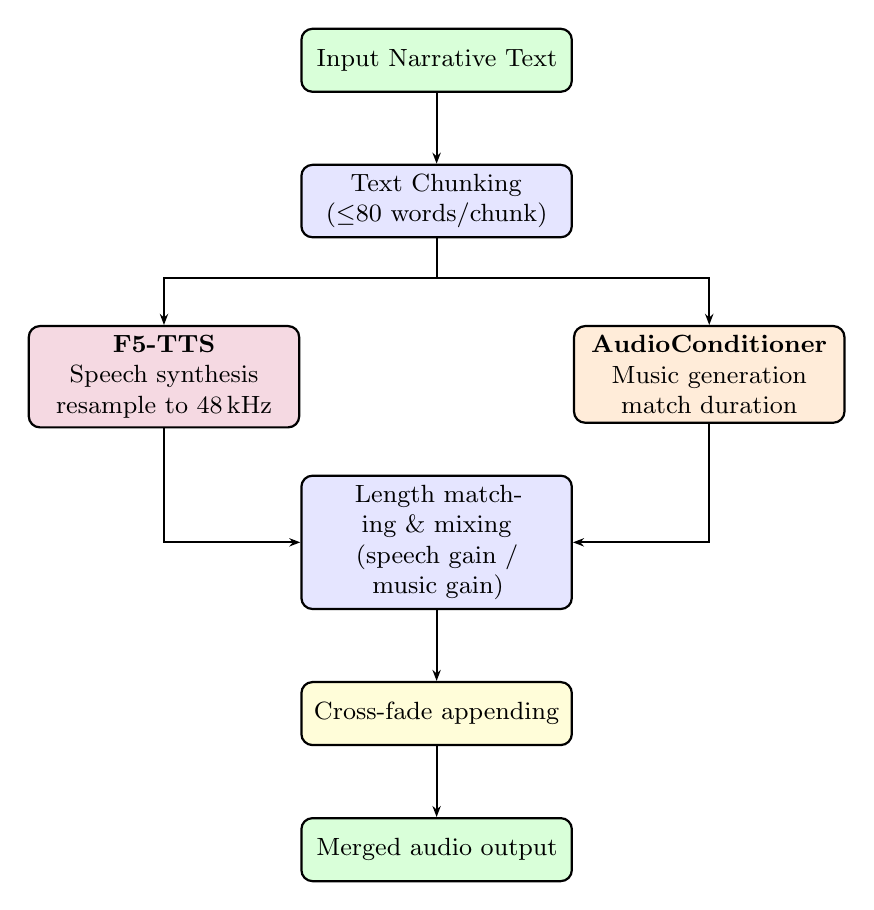
\begin{tikzpicture}[
    node distance=0.9cm and 0.8cm,
    box/.style={rectangle, draw=black, thick, fill=blue!10,
                text width=3.2cm, align=center, rounded corners,
                minimum height=0.8cm, font=\small},
    arrow/.style={-{Stealth[length=4pt]}, thick}
]
    \node[box, fill=green!15] (input) {Input Narrative Text};
    \node[box] (chunking) [below=of input] {Text Chunking\\($\le$80 words/chunk)};

    \node[box, fill=purple!15] (tts) [below left=1.1cm and 0cm of chunking]
        {\textbf{F5-TTS}\\Speech synthesis\\resample to 48\,kHz};
    \node[box, fill=orange!15] (ac) [below right=1.1cm and 0cm of chunking]
        {\textbf{AudioConditioner}\\Music generation\\match duration};

    \node[box] (mixer) [below=3.0cm of chunking]
        {Length matching \& mixing\\(speech gain / music gain)};
    \node[box, fill=yellow!15] (fade) [below=of mixer] {Cross-fade appending};
    \node[box, fill=green!15] (output) [below=of fade] {Merged audio output};

    \draw[arrow] (input) -- (chunking);
    \draw[arrow] (chunking.south) -- ++(0,-0.5) -| (tts.north);
    \draw[arrow] (chunking.south) -- ++(0,-0.5) -| (ac.north);
    \draw[arrow] (tts.south) |- (mixer.west);
    \draw[arrow] (ac.south) |- (mixer.east);
    \draw[arrow] (mixer) -- (fade);
    \draw[arrow] (fade) -- (output);
\end{tikzpicture}}
\caption{ReadMusic per-chunk pipeline. Speech and music are generated in
parallel per chunk, mixed with fixed gains, and appended with a short
crossfade to produce a continuous narrated audiobook.}
\label{fig:readmusic_pipeline}
\end{figure}

The narrative is split at natural boundaries (punctuation, newlines) into chunks of at most 80~words -- imposed by Stable Audio Open's 47-second generation ceiling.
For each chunk, F5-TTS synthesis and AudioConditioner music generation run concurrently.
The resulting waveforms are zero-padded to equal length, multiplied by configurable speech and music gains, and concatenated with a short crossfade to avoid abrupt transitions between chunks.
For long-form narratives (\eg Grimm's fairy tales), the Phase-2 fine-tuned checkpoint is used so that consecutive MusicDescriptor predictions maintain a temporally coherent emotional arc.

\section{Application III: Image-to-Video with Soundtrack}
\label{app:video}

\texttt{video\_sound.py} creates a short cinematic clip with a synchronized score from a single input image.
The two generation streams run in \textbf{parallel} (\cref{fig:video_pipeline}):

\begin{figure}[h]
\centering
\scalebox{0.75}{%
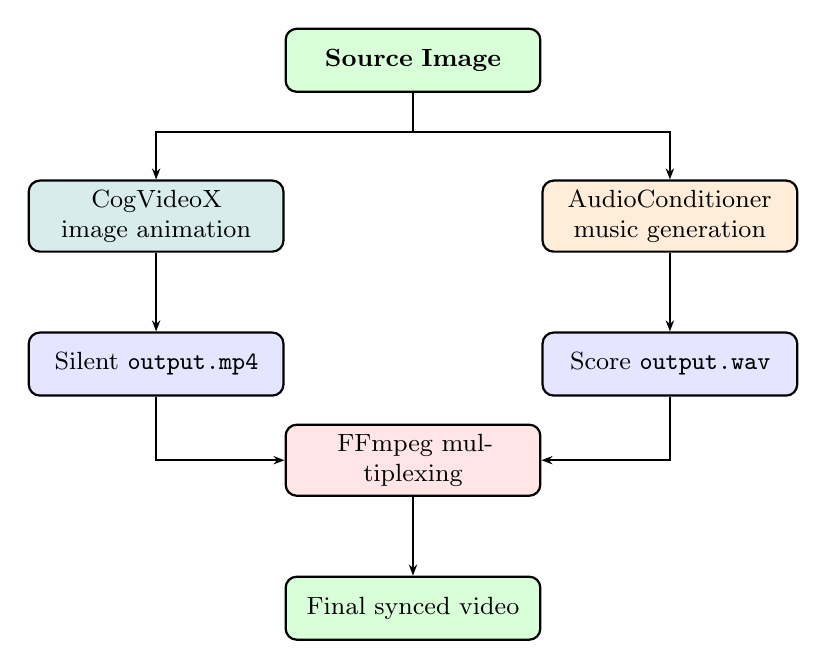
\begin{tikzpicture}[
    node distance=1.0cm and 0.5cm,
    box/.style={rectangle, draw=black, thick, fill=blue!10,
                text width=3.0cm, align=center, rounded corners,
                minimum height=0.8cm, font=\small},
    arrow/.style={-{Stealth[length=4pt]}, thick}
]
    \node[box, fill=green!15] (img) {\textbf{Source Image}};

    \node[box, fill=teal!15] (vid)  [below left=1.1cm and 0cm of img]
        {CogVideoX\\image animation};
    \node[box, fill=orange!15] (aud) [below right=1.1cm and 0cm of img]
        {AudioConditioner\\music generation};

    \node[box] (vf) [below=of vid]  {Silent \texttt{output.mp4}};
    \node[box] (af) [below=of aud]  {Score \texttt{output.wav}};

    \node[box, fill=red!10] (ffmpeg) [below=4.2cm of img]
        {FFmpeg multiplexing};
    \node[box, fill=green!15] (final) [below=of ffmpeg]
        {Final synced video};

    \draw[arrow] (img.south) -- ++(0,-0.5) -| (vid.north);
    \draw[arrow] (img.south) -- ++(0,-0.5) -| (aud.north);
    \draw[arrow] (vid) -- (vf);
    \draw[arrow] (aud) -- (af);
    \draw[arrow] (vf.south)  |- (ffmpeg.west);
    \draw[arrow] (af.south)  |- (ffmpeg.east);
    \draw[arrow] (ffmpeg) -- (final);
\end{tikzpicture}}
\caption{Image-to-video pipeline. CogVideoX animates the image while
AudioConditioner generates a matching score; FFmpeg muxes the two streams
into a final video file.}
\label{fig:video_pipeline}
\end{figure}

\begin{enumerate}
  \item \textbf{Image animation.} CogVideoX~\cite{yang2024cogvideox} (image-to-video diffusion) generates a short silent clip from the input image. As an open-weight model, video quality is limited but sufficient as a proof-of-concept.
  \item \textbf{Score generation.} AudioConditioner simultaneously processes the same image through BLIP captioning, descriptor prediction, and Stable Audio Open synthesis to produce a matching audio waveform.
  \item \textbf{Multiplexing.} FFmpeg muxes the silent video and the generated audio into a single file, trimming or padding to a common duration.
\end{enumerate}

No additional training is required; the two generative pipelines operate independently and are combined purely at the file level.
Visible artifacts in the animated video are expected at the current open-weight model scale; audio quality is markedly higher and constitutes the primary perceptual contribution of the application.

\end{document}
